\subsection{Anwendungsbereiche}
\subsubsection{Recherchegrund}
Wir wollen wissen, ob und welche Abwasserkraftwerksysteme bereits bestehen. Gibt es auch Systeme für die Energiegewinnung via Abwasserturbinen in Hochhäusern? Wie sieht deren Markt aus? Gibt es abgesehen vom Hochhaus noch andere Bereiche, die mit unserem System abgedeckt werden könnten?
\subsubsection{Ergebnisse}
\paragraph{Abwasserkraftwerksysteme}
Grosse Wasserkraftwerke (ca. 100\si{MW}) brauchen viel Platz (grosse Dämme und lange Kanäle) und haben einen unvorhersehbaren Effekt auf Flora und Fauna. Deshalb erscheint die Entwicklung und Realisierung von Kleinkraftwerken (ca .100\si{kW}) umso wichtiger. Die Entwicklung von Abwasserkraftwerksystemen spielt dabei eine grosse Rolle. Folgende erforschte und oder bestehende Systeme konnten gefunden werden:
\paragraph{Kanalisation zwischen Stadt und Kläranlage}
Wenn in den Abwasserrohren zwischen einer Stadt und deren Kläranlage ein hydraulisches Potential vorliegt, könnte dieses durch Turbinen genutzt werden. Bereits 1992 wurde in Le Châble eine Pelton-Turbine eingesetzt, um das Abwasser vom höher gelegenen Ferienort Verbier zu nutzen(LINK). In Japan wurde in der Gegend des Toyogawa Flussbeckens untersucht, wo hydraulische Potentiale in den Abwasserrohren bestehen. Zudem wurden drei kleine Turbinen mit unterschiedlicher Beschaufelung auf Verstopfung durch Fremdmaterial untersucht. Die Studie (LINK) schliesst mit einem positiven Ergebnis.
\paragraph{Abfluss von Kläranlagen}
"Electricity is the second largest operating cost at WWTPs [Kläranlagen¨], representing 25 to 40\% of the total operating budget."
Aus diesem Grund sind viele Kläranlagen (z.Bsp. Aquarion Water Co (USA) und North Head WWTP (AUS)) darum bemüht, ihre Energiekosten zu reduzieren. In Australien wurde dies in einem Pilotprojekt bereits realisiert, indem das hydraulische Potential genutzt wurde, das zwischen der Kläranlage und dort, wo das gereinigte Wasser hinfliesst, besteht. Das dort verwendete Turbinensystem (Flow-to-Wire) (LINK) wurde von der amerikanischen Firma Rentricity hergestellt. Der Vorteil von dieser Variante ist, dass das Problem der Verstopfung duch das bereits gereinigte Wasser ausbleibt.
Ähnliche Systeme für Trinkwasserleitungen existieren bereits in Oregon und Kalifornien (LucidPipe LINK). Aber auch hier wird erwähnt, dass ein grosser Wasserstrom (53 Mio. Liter pro Tag) nötig ist, damit sich eine Installation lohnt.
\paragraph{In Hochhäusern}
Es wurde nur ein Pilotprojekt (HighDro Power, Tom Broadbent) gefunden, wo eine Abwasserturbine für die Anwendung innerhalb von Gebäuden entwickelt wurde.
\begin{figure}[h!]
  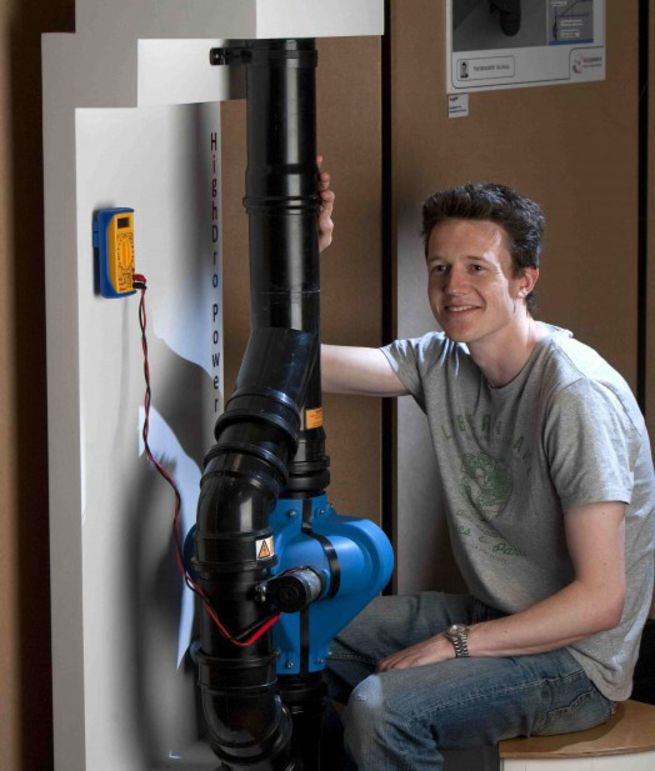
\includegraphics[width=7cm]{highDro.jpg}
  \caption{Tom Broadbent and his turbine.}
  \label{fig:turbineTomBroadBent}
\end{figure}
Die Trinkwasserversorgung der obersten Stockwerke eines Hochhauses erfordert viel Druck (6-8 Bar). Da dieser Druck für die unteren Stockwerke zu gross ist, werden da Druckreduzierventile eingesetzt. Dabei bleibt viel Energie ungenutzt. Für diese Anwendung existieren schon Lösungen (z.Bsp. Arup LINK). Aber:
"Small-scale systems cannot easily generate enough power to justify their cost to large developers. The price per kilowatt-hour of generating power can be five times as high as simply buying it from the grid."(NEWYORKTIMES LINK)
\subsubsection{Fazit}
\clearpage 
